\documentclass{article}
\usepackage{graphicx} % Required for inserting images
\usepackage{url}
\usepackage{tikz}
\usepackage{hyperref}

\graphicspath{{./diagram/}}

\title{MA-Proposal-Danesh}
\author{Navid Rahimidanesh}
\date{March 2023}

\begin{document}

\maketitle

\section{Abstract}

\section{Introduction} % 1.5 Page

\subsection{Motivation}

\subsection{Thesis Goal}

Towards a data sharing platform for "Cyber Threat Intelligence" information focused on the Smart Grid use case, that supports privacy and sovereignty of data to increase the security of smart electricity infrastructure.

\subsection{Outline}


\section{Background and Related Work} % 4 pages

\subsection{Background}
\subsubsection*{Smart Grid Security}
A smart grid is an advanced electrical grid that uses advanced technologies to efficiently manage the generation, distribution, and consumption of electricity. Smart grid security involves protecting the system from cybersecurity threats that can disrupt or damage the grid's operations. It could be divided into three layers: physical security, network security, and data security. Physical security includes measures to protect the physical infrastructure of the grid, such as substations, transformers, and power lines. This can include fencing, security cameras, and access controls. Network security involves protecting the communication networks used by the smart grid. This can include implementing firewalls, intrusion detection systems, and encryption to prevent unauthorized access or attacks. Data security involves protecting the data generated and used by the smart grid, including customer data, operational data, and control data. This can include implementing access controls, data encryption, and backup and recovery systems to ensure the availability and integrity of the data. 


Smart grids face a range of severe cyber threats, including data injection attacks on state estimation [5,6], distributed denial of service (DDoS) and denial of service (DoS) attacks [7], targeted attacks, coordinated attacks, hybrid attacks, and advanced persistent threats [8,9]. Moreover, in recent years, ransomware campaigns have emerged as a significant risk to the sector [10-12].



\subsubsection*{Threat intelligence Sharing}
Cyber threat intelligence (CTI) is the process of collecting, analyzing, and disseminating information about potential or current cyber threats. CTI relies on gathering data from diverse sources, including security tools, threat feeds, honeypots, forums, social media platforms, and other relevant online and offline sources. This data can include indicators of compromise (IOCs), malware samples, network traffic logs, vulnerability information, and more. The goal is to provide organizations with a comprehensive understanding of potential cyber threats to make informed decisions. It helps identify the tactics, techniques, and procedures (TTPs) used by threat actors and vulnerabilities in an organization's security infrastructure. It is an important component of a comprehensive cybersecurity strategy to reduce the risk of a cyber attack. Sharing cyber threat intelligence allows organizations to enhance their situational awareness, proactively defend against potential threats, and improve incident response capabilities. Through collaboration and information exchange between organizations, it leads to a more robust cybersecurity posture for the entire community.

There are several approaches and frameworks for sharing CTI, including commercial and non-commercial platforms. It could include government initiatives as well as open-source communities. Commercial platforms are typically managed by cybersecurity vendors that provide CTI feeds to their customers. Non-commercial platforms include collaborative initiatives among organizations, such as Information Sharing and Analysis Organizations (ISAOs) and Information Sharing and Analysis Centers (ISACs).

Despite the benefits of CTI sharing, there are also gaps and limitations that need to be addressed. These include concerns around privacy, legal and regulatory barriers, lack of trust among participants, and difficulties in sharing information in real-time. In addition, the lack of a standardized format for CTI sharing can make it challenging for organizations to share and use CTI effectively. As such, efforts to standardize CTI sharing formats and improve trust among participants are critical for improving the effectiveness of CTI sharing initiatives.

\subsubsection*{Data Modeling}
In the context of CTI sharing, data modelling serves three purposes: (1) to provide a backbone for all relevant information, (2) to specify the data input format for further analysis, (3) to define the desired target for information gathering. \cite{husak_crusoe_2022}

Heterogeneous data formats from different incompatible security tools.

\subsubsection*{Data Spaces}
The term data spaces term was first coined by Franklin et al to describe a new paradigm for data management \cite{franklin_databases_2005}. It solves some data integration tasks by offering a consolidated perspective of data residing in diverse origins, encompassing databases, files, and web services without physically transfer the data. He proposed a DataSpace Suppport Platform (DSSP) that helps developers by enabling them to query and manipulate the data from multiple sources using a single query language with the help of this unified view of data sources.

Beside its technological definition, one could define data spaces from an economic point of view, where data spaces is a form of data exchange. In this viewpoint, dataspaces describes a situation where two or more organizations exchange data to gain a common benefit. \cite{reiberg_what_2022}

However, there is not a single definition of data spaces. Dataspaces is a concept to fulfill several requirements. In different contexts, different requirements are more important than others. 

Data sharing or integration is one requirement. Data spaces could be used to integrate data from different sources. It could also be viewed as a data exchange platform in some contexts.

Another crucial requirement, that makes data spaces interesting, is the sovereignty of data. Sovereignty can generally be defined as supreme authority. In the context of data, it denotes the right of the owner to control how and by whom will the data be used. Data spaces could fulfill this requirement by keeping the data in the data source and providing a unified view of the data to the consumers with respect to the access control policies defined by the owner of the data.

Another aspect of data spaces is its governance. It is required to define a set of policies, rules and protocols to ensure a smooth exchange of data. Therefore, a governance body is expected to be established to define and enforce these policies. \cite{reiberg_what_2022}

Data spaces should be open, meaning anyone complying with the policies should be able to join without restriction. This encourages a fair and non-monopolistic market. This entails an easy access, which means, anyone could be able to connect with a limited effort.

Data spaces are usually designed to be decentralized and federated. Meaning there is no entity having direct control over all data exchanges. Different participants could interact with each other directly. This emphasizes the role of interoperability. This is only possible when certain open standards are established. Consequently, data spaces complying to the same standards could be embedded inside each other enabling cross-data-space exchange \cite{reiberg_what_2022}.

\noindent\fbox{%
    \parbox{\textwidth}{%
    "Data Spaces are defined as: A federated, open infrastructure for sovereign data sharing, based on common policies, rules and standards." \cite{reiberg_what_2022}
    }%
}

\subsection{Related Work}

\subsubsection*{EE-ISAC}
European Energy Information Sharing and Analysis Centre (EE-ISAC) is a non-profit organization that facilitates the exchange of cyber threat information between its members. Since its foundation in 2015 it acquired over 30 members from utilities, academia, governmental and non-governmental organizations. Members exchange cyber threat information through plenary meetings, working groups, and a dedicated platform (based on MISP). EE-ISAC facilitates trust based information exchange which is not present in the mandatory information sharing in the NIS directive. This trust is achieved by confidentiality agreements and regular physical meetings with the same members. 
\cite{wallis_ee-isacpractical_2022}

\subsubsection*{IDS}
The International Data Spaces (IDS) is an initiative with the goal of creating a standard for a distributed software architecture for data exchange with sovereignty. It was launched in 2015 as a Fraunhofer research project funded by the German Federal Ministry for Education and Research \cite{otto_evolution_2022}. Shortly after that, in 2016, the IDS Association (IDSA) was founded as a non-profit organization to continue the research. It resulted in definition of the IDS Reference Architecture Model (IDS RAM). The IDS RAM is the description of IDS components and their interactions without being technology specific \cite{otto_evolution_2022}. IDS RAM allows anyone to implement the IDS compliant components using any technology. The IDSA also provides a reference implementation of different IDS components called IDS Testbed \cite{noauthor_ids_2022}. 

IDS RAM defines the following components \cite{pettenpohl_international_2022}:
- Connector: The connector is the interface between the IDS ecosystem and the data source. It is responsible for the data exchange and the enforcement of the usage control policies as well as authentication.
- Identity Provider: authentication service managing identity information
- IDS Broker: Manages the metadata (description and usage policies)
- Clearing House: Audits the data exchange and manages the payment
- IDS Apps: Process the exchanged data. Deployed within Connector.
- App Store: Provides IDS apps
- Vocabulary Provider: Offers vocabularies to describe and annotate data

Furthermore, the participants could undertake different roles \cite{pettenpohl_international_2022}:
- Data Owner: Controls the data and defines usage policies and payment model.
- Data Provider: Provides the data to the IDS ecosystem with respect to the policies defined by the data owner.
- Data Consumer: Same as data provider but consumes the data.
- Data User: Same as data owner but uses the data.
- App Provider
- ...


Usage Control:

Certification:



\subsubsection*{Gaia-X}
European data strategy Towards a single market of data. + technological independence of Europe. No vendor lock-in. Launched in 2019. Sovereign digital ecosystem
Gaia-X is an initiative that aims to foster generation of a data and service infrastructure by developing regulations and technical specifications which is based on European values, applicable to any existing cloud and edge technology stack. Gaia-X allows for transparency, controllability, portability and interoperability across data and services. It will ease value creation through data collection and sharing between organizations leading to a vibrant data ecosystem across Europe and beyond. Gaia-X Association deliverables include federation services, common policy rules and an architecture of standards. (Data sovereignty?) Federation services could be utilized by the ecosystem participants to achieve a global interoperability, compliance and effortless set up. This includes, "Identity and Trust", "Federated Catalog" and "Data Exchange services". \cite{otto_role_2022}
AISBL: Gaia-X Association
Nodes, Services (Any cloud service), Service Instances (A service running on a node) and Data Assets (a data set on a node)
Participants: Organizations and individuals that are part of the Gaia-X ecosystem
Clearing House: Middle man in the exchange checking for compliance

\subsubsection*{Comparison of IDS and Gaia-X}
Gaia X 2019, IDS 2015. IDS is more mature. it is already tested in the industry. Gaia X is still in the development phase.
Gaia X offers a more holistic approach including cloud elements.
Gaia X is more focused on cloud services. IDS is more focused on data exchange.
Gaia X is more focused on the business and economic side. IDS is more focused on the technical side.
Gaia-X could use IDS as a component \cite{otto_role_2022}
Gaia-X provides standards for infrastructures and cloud elements. IDS provides standards for data exchange.
Federated Catalog ~ IDS Broker + Vocabulary Provider + Information Model
Identity and Trust ~ IDS Identity Provider + Dynamic Attribute Provisioning Service (DAPS)
Gaia X Sovereign Data Exchange ~ IDS Usage Control and Clearing House
Gaia X Node ~ IDS Connector

- Documentation: 
- Maturity: Gaia-X is still in the development phase. IDS is more mature.
- Implementation: IDS is open source and has a reference implementation. Gaia-X is not open source and does not have a reference implementation.



\subsubsection*{Other Platforms}
Platform Industrie 4.0, 
SWIPO: is an association that develops and safeguards codes of conduct to facilitate Switching and Porting of non-personal data between cloud providers and their customers.
It follows the Free Flow of Non-Personal Data regulation.

\subsubsection*{Crowd Sourced Sharing}
The sharing is caring paper \cite{jesus_sharing_2023}

% ---------------------------------------------------------------

\section{Use case and Requirements} % 3 Pages
Scenario
Requirements
Constraints

Two motivations for usage control:
- Internal: 
- External: EU-GDPR

% Stake-holders (Actors) and their profile
% - Utility Provider
% - Utility Operator
% - BSI (in Germany)
% - SOC (Different levels)

- Confidentiality
- Security
- Do we need plausible deniability?
- Combat against free-riding
- Trust and reputation


\section{Conceptual Approach} % 1.5 Pages

Components and relation to requirements
Discuss Benefits and limitations
Compare with existing solutions

\begin{figure}[h]
    \centering
    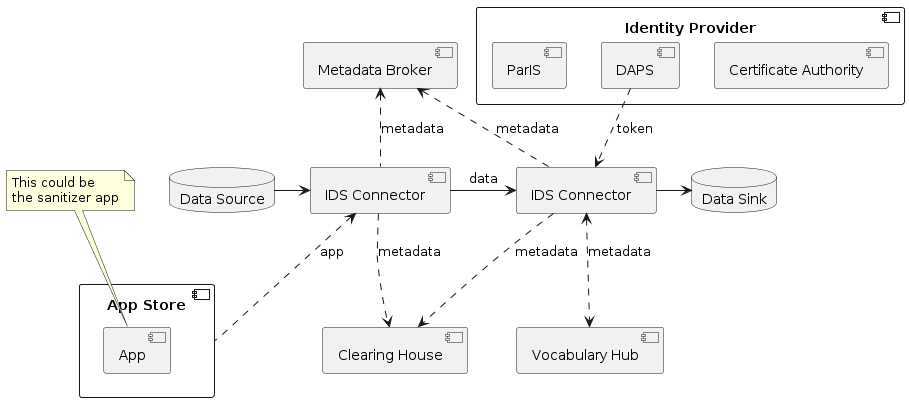
\includegraphics[width=\textwidth]{components}
    \caption{System Architecture Diagram}
    \label{fig:system-architecture}
\end{figure}

Important data space components that are relevant to our use case are listed below. The descriptions fully conform to the IDSA RAM 4.0 \cite{otto_ids_2019}.
\begin{itemize}
    \item Connector: It is the primary component involved in the data exchange acting either as data provider or consumer. Not only it performs the actual data exchange but also the enforcement of the usage control policies as well as authentication. It can be operated on-premises or in a cloud environment. It will run the IDS Apps that do process the data among other things (more on that later). It uses application container management technology to isolate data apps and core functionalities.
    \item IDS Broker: The IDS Metadata Broker is an IDS Connector, which contains an endpoint for the registration, publication, maintenance, and query of Self-Descriptions. Self-Descriptions encapsulate information about Connectors, their managing participant, the offered data assets, and the respective usage conditions. In a sense, the IDS Broker is like a phonebook.
    \item Identity Provider: This is the component serving as Identity and Access Management (IAM). It's responsible for assigning identities to participants, verifying identity claims and granting access based on identities. It comprises three components: 
        \begin{itemize}
            \item CAs: One or multiple certificate authorities are responsible for issuing certificates to participants upon request. They are also responsible for revoking certificates. They are the trust anchors by which all other components can be verified.
            \item Dynamic Attribute Provisioning Service (DAPS): It complements the certificates issued by CAs with more volatile attributes in form of tokens. Connectors can request Dynamic Attribute Tokens (DATs) from DAPS to prove their attributes to other components.
            \item Participant Information Service (ParIS):  It provides business-related information about participants in the IDS that have been checked by the Support Organization. Similar to the way Broker provides metadata about data assets, ParIS provides metadata about participants.
        \end{itemize}
    \item Clearing House: It is a trusted third party in the data exchange that logs all the required information about clearing, billing, and usage control. It keeps track of the payment information and also usage information to help verify the compliance with the usage policies.
    \item IDS Apps: These are re-usable software components that can be deployed inside the IDS Connector. They are mainly used to transform or analyze data. However, they can also be used to connect to enterprise services, or to allow the connector to be controlled by external systems. Data apps can be chained and bundled.
    \item App Store: As the name suggests, it is a marketplace for IDS Apps. It contains endpoints to publish, search, and download IDS Apps. It is a Connector on its own, so it should pass the IDS certification criteria and provide a self-description.
    \item Vocabulary Provider: To facilitate cooperation of different IDS components, a common vocabulary is required. The vocabulary provider enables the participants to define and publish their own vocabularies. Vocabularies typically follow the RDF standard. An example usage is to reference an RDF URI in the Self-Description of a data asset.
\end{itemize}

Apart from the components described by the IDS RAM, there are other components that are not part of the IDS RAM but are relevant to our use case. These components are described below.

\begin{itemize}
    \item Sanitization App: This is an IDS App that is responsible for sanitizing the data. It is deployed inside the IDS Connector. It is responsible for removing the sensitive information from the data before it is shared with other participants. IDS App is suitable for this task because dealing with sensitive data requires a high level of trust. Apps are certified and verified by the App Store. Furthermore, they are executed within the Connector, so they have access to the data before it is shared with other participants. This is important because it prevents the data from being leaked before it is sanitized. 
\end{itemize}

\section{Realization / Implementation} % 1 Page
% Which technology and tools you use?
% Architecture
% - Which parts will you implement yourself, and which part you copy?
%     - IDS Testbed
%     - 

% - How they fit with dataspace components?

\subsection*{IDS Connector}
The IDS Association publishes a monthly report of the current state of all the data connectors used for exchange of data, not limited to the IDS compliant connectors.
 Dam et al. \cite{dam_survey_2023} investigated this report and published a survey in September 2023. They found that only 4 connectors have their source code available on a public repository: 1) IDS Dataspace Connector (DSC) by sovity, Eclipse Dataspace Connector (EDC), the TRUsted Engineering (TRUE) Connector, and the Trusted Connector by Fraunhofer AISEC.

In addition to that, I found two more: First, IDS Integration Toolbox by Open Logistics Foundation which is a wrapper around the DSC. Second, TNO Security Gateway (TSG) initially developed by TNO which has implementations for many IDS components. It is used in Smart Connected Supplier Network (SCSN) data space and has a documentation.
However, it has no stars on gitlab.

The overview of different conenctors is shown in table \ref{tab:connectors}.

\begin{table}[ht]
    \label{tab:connectors}
    \centering
    \begin{tabular}{| c c c c c c|}
    \hline
    \textbf{Name} & \textbf{Created} & \textbf{Stars} & \textbf{Commits} & \textbf{Last Release} & \textbf{Hosted} \\
    \hline
    \hline
    DSC & 07.10.2020 & 27[+101] & 2600 & 10.22 & \href{https://github.com/International-Data-Spaces-Association/DataspaceConnector}{Github} \\
    \hline
    EDC & 13.01.2021 & 202 & 1817 & 10.23 & \href{https://github.com/eclipse-edc/Connector}{Github} \\
    \hline
    TRUE & 30.10.2020 & 19 & 122 & 08.23 & \href{https://github.com/Engineering-Research-and-Development/true-connector}{Github} \\
    \hline
    Trusted & 05.09.2017 & 43 & 2221 & 02.23 & \href{https://github.com/Fraunhofer-AISEC/trusted-connector}{Github} \\ 
    \hline
    Toolbox & 31.03.2022 & 3 & 172 & 04.23 & \href{https://git.openlogisticsfoundation.org/silicon-economy/base/ids/ids-integration-toolbox}{Self-Hosted} \\
    \hline
    TSG & 12.05.2021 & 0 & 243 & 08.23 & \href{https://gitlab.com/tno-tsg}{Gitlab} \\
    \hline
    \end{tabular}
    \caption{Available IDS Connectors}
\end{table}

Most number of stars and most recent release being a deciding factor, I will choose EDC to base my implementation on.

\subsection*{IDS Testbed}
The IDS association defines Minimum Viable Data Space (MVDS) as the minimum set of components that provide the ability to do secure and sovereign data exchange. They specify the required components as follows: Two Connectors (a data provider and a consumer), an Identity Provider (Dynamic Attribute Provisioning Service, Certificate Authority). IDSA has published an open-source project, \href{https://github.com/International-Data-Spaces-Association/IDS-testbed}{IDS Testbed}, that contains instructions to install and orchestrate these set of minimum components. It references open-source implementations of these components, see table \ref{tab:components} to find source code of these components.

\begin{table}[h]
    \label{tab:components}
    \centering
    \begin{tabular}{|c|c|c|c|}
    \hline
    \textbf{Component} & \textbf{Source Code} & \textbf{Version} & \textbf{Language} \\
    \hline
    IDS Testbed & \href{https://github.com/International-Data-Spaces-Association/IDS-testbed}{Testbed Git} & 1.0 & Docker-Compose \\
    \hline
    Connector & \href{https://github.com/International-Data-Spaces-Association/DataspaceConnector/tree/v8.0.2}{Connector Git} & 8.0.2 & Java \\
    \hline
    Metadata Broker & \href{https://github.com/International-Data-Spaces-Association/metadata-broker-open-core}{Broker Git} & 5.0.3 & Java \\
    \hline
    DAPS & \href{https://github.com/International-Data-Spaces-Association/omejdn-daps}{DAPS Git} & 1.6.0 & Ruby \\
    \hline
    Certificate Authority & \href{https://github.com/International-Data-Spaces-Association/IDS-testbed/tree/master/CertificateAuthority}{Testbed Git} & --- & Python \\
    \hline
    App Store & \href{https://github.com/International-Data-Spaces-Association/IDS-AppStore}{App Store Git} & 3.0.0 & Java \\
    \hline
    \end{tabular}
    \caption{Necessary Components}
\end{table}

In addition to the aforementioned components, some new ones need to be implemented from scratch: App Store, ParIS, Clearing House, Vocabulary Hub. Of course, the required IDS Apps should be implemented, which includes, the Sanitization App. 
For the App Store there is a published project (\href{https://github.com/International-Data-Spaces-Association/IDS-AppStore}{App Store Git}) which is not included in the testbed and might not be fully functional.

\subsection*{Usage Policies}
To describe usage policies IDS defines its own Usage Control Language which is an extension of Open Digital Rights Language (ODRL). It is a machine readable format which is technology agnostic. There are multiple mechanism to enforce these policies automatically. The position paper on IDS Usage Control \cite{eitel_usage_2021} lists the following mechanisms: MYDATA Control Technologies, Logic based Usage Control (LUCON), and Degree (D°). According to the paper, MYDATA Control Technologies is the most mature and comprehensive. It is also the only one that is implemented in the IDS Testbed. Therefore, I will use MYDATA Control Technologies to enforce the usage policies. The usage control is enforced in the IDS Connector possibly using a separate application container. It comprises three different components: PMP, manages policies and creating them based on some templates, PDP, evaluates the policies and decides whether to allow or deny the request, and PEP, enforces the decision made by PDP. The overview of the components is shown in figure \ref{fig:connector}.

\begin{figure}[h]
    \centering
    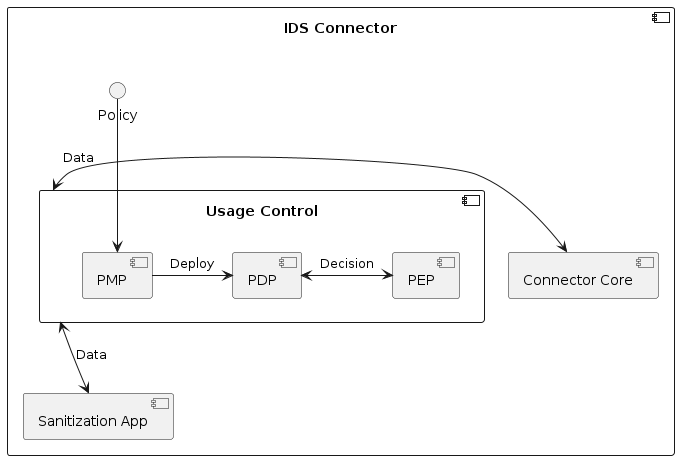
\includegraphics[width=\textwidth]{connector}
    \caption{Connector Overview}
    \label{fig:connector}
\end{figure}


\subsection*{Sanitization App}
Removing all sensitive data from CTI in general can be a difficult task. There are different CTI formats and each format has its own structure. Furthermore, deciding whether a value contains confidential information or not is not straight-forward. Even a sophisticated machine learning approach requires a lot of data with different types of confidential information to be trained on. Therefore, I will focus on creating a base sanitization app that is easily extensible to detect more sensitive data. To start, it should support sanitizing JSON based CTI formats, and a configurable set of regex rules to detect sensitive data. Refining this app to support more formats and more sophisticated detection mechanisms is out of scope of this thesis.

\section{Evaluation} % 0.5 Page
% Methodology and Metrics
% Test scenario

% - How to gather (CTI) data?
% - Metrics for evaluating the privacy? (e.g. entropy)
% - The steps of the scenario and the expected results
% - How to measure the performance?

My contribution being design of a sharing platform for CTI data, the evaluation should measure the effectiveness of the sharing platform. The problem is that according to my research, there is no benchmark available and no defined metrics to this aim. Having no baseline to compare against, it seems hard to reach an objective evaluation. Furthermore, many performance metrics depend on the implementation, infrastructure, and the details of the scenario. Since, my main contribution is the design of the platform, not the implementation, some metrics can be misleading. 

However, several options can be thought of. First, by focusing on the main effect of using data spaces for data sharing, which is the addition of usage control and changing the data flow, one can define a few specific metrics. Having defined some usage case scenarios and a sample implementation, we can measure for example the following metrics: 
\begin{itemize}
    \item Number of unnecessary participants that should have access to the data.
    \item The difficulty of changing the usage policies.
    \item How difficult it is to revoke access to the data.
    \item Variety of types of usage policies that are enforceable.
    \item How many scenarios are significantly improved using our approach.
\end{itemize}

The above-mentioned items might be subjective and change by modifying the chosen scenarios, but investigating it can provide some insights into the effectiveness of the data spaces.

Another approach which can sound more objective is to design a survey. It should use some standard templates to be comparable. The survey should be conducted on a group of experts in the field of CTI sharing after presenting them our approach. The survey should be designed to measure the effectiveness of our design in terms of privacy and security. Ideally, 10 to 20 experts should be interviewed. There is a risk of not having enough experts available. In that case, we fall back to the first approach.


\section{Timeline / Milestones / Project Plan} % 0.75 Page

\bibliography{ref} 
\bibliographystyle{ieeetr}

\end{document}
